\section{Methodology}

In this section, we introduce the ReSum paradigm, the development of ReSumTool-30B, and the ReSum-GRPO algorithm designed to facilitate paradigm adaptation.

\subsection{ReSum Paradigm}
\textbf{Trajectory Initialization:} The trajectory begins with a user query $q$, initializing $\mathcal{H}_0 = (q)$. Following ReAct, the agent alternates between internal reasoning and tool use: at the $t$-th round, it generates a reasoning step within \think{} tokens and issues a tool call within \search{} tokens, expressed as $(\tau_t, a_t) \sim \pi_{\theta}(\cdot \mid \mathcal{H}_{t-1})$. The system parses the tool call arguments and executes the corresponding tool, returning results within \response{} tokens as $o_t = \mathcal{R}(a_t)$, where $\mathcal{R}$ represents the tool environment. The history is then updated by concatenation as follows:
\[
\mathcal{H}_t \,=\, \mathcal{H}_{t-1} \circ (\tau_t, a_t, o_t).
\]
In the initial rounds, ReSum mirrors ReAct by iteratively building $\mathcal{H}_t = \left( q, \tau_1, a_1, o_1, \ldots, \tau_t, a_t, o_t \right)$.

\textbf{Context Summarization:} When a compression trigger is activated, a summary tool $\pi_{\text{sum}}$ is invoked to summarize the accumulated history as:
\[
s \sim \pi_{\text{sum}}(\cdot \mid \mathcal{H}_t),
\]
where $s$ is a goal-oriented \textbf{\summary{}} that consolidates essential evidence (prompt provided in Appendix \ref{appendix:prompt}). Then, we form a compressed state $q' = (q, s)$ and reset the working history to:
\[
\mathcal{H}_t \leftarrow (q').
\]

Summarization can be triggered \emph{\textbf{systematically}}, e.g., hitting token limits, or \emph{\textbf{autonomously}} by the agent. In this work, we adopt systematic triggers to ensure predictable behavior, as reliable self-initiated context management often exceeds the capabilities of current agents.

\textbf{Trajectory Termination:} Through periodic summarization, ReSum dynamically maintains the context within the model's window while preserving essential evidence. The agent continues gathering evidence and, once sufficient information is accumulated, produces a synthesized answer within \answer{} tokens. Although ReSum theoretically allows unbounded exploration, practical deployments impose resource budgets, e.g., limiting the number of tool calls. Trajectories that exceed these limits are terminated and marked as failures.

The ReSum execution flow is detailed in \textbf{Algorithm \ref{alg:resum_rollout}} in Appendix. By transforming linear interaction histories into restartable and compact states, ReSum enables long-horizon exploration that would otherwise overflow the context window, while maintaining functional compatibility with existing ReAct-based agents.


\subsection{Summary Tool Specification}

In ReSum, an off-the-shelf LLM can serve as the summary tool. However, its role extends far beyond conventional conversation summarization. To guide web agents in persistent, goal-oriented exploration, the summary tool must perform logical reasoning over lengthy and noisy interaction histories, distill verifiable evidence from large text snippets, and propose actionable, well-scoped next steps grounded in web context. These capabilities typically exceed those of small generic models that lack web-context reasoning, while large reasoning models incur prohibitive inference latencies and costs. To bridge this gap, we develop \textbf{ReSumTool-30B} through a rigorous three-stage pipeline.

\textbf{Teacher Model Selection:} We first conducted an empirical study comparing models of varying scales in Appendix~\ref{appendix:summary_case}. Our analysis reveals that reasoning-enhanced models outperform instruction-tuned counterparts in structured evidence synthesis and source attribution. Therefore, we select GPT-OSS-120B~\citep{gpt-oss} as the teacher model for its superior ability to maintain goal consistency over long horizons.

\textbf{Data Synthesis:} We construct our training data by recording the ReSum trajectories on the \textbf{SailorFog-QA} benchmark~\citep{li2025websailor}, which mirrors challenging real-world tasks requiring long-horizon reasoning. In this setup, we decouple the exploration and summarization roles to ensure quality: a WebSailor agent serves as the explorer, leveraging its persistent information-seeking capabilities to navigate and gather context, while the teacher model is integrated as the summary tool. This process yields over 9,000 high-quality $\langle \texttt{Conversation}, \texttt{Summary} \rangle$ pairs. 

\textbf{Development:} Leveraging these collected pairs, we distill the teacher model's capability into Qwen3‑30B-A3B-Thinking\footnote{\href{https://huggingface.co/Qwen/Qwen3-30B-A3B-Thinking-2507}{https://huggingface.co/Qwen/Qwen3-30B-A3B-Thinking-2507}}, selected for its MoE architecture that enables efficient deployment while maintaining strong reasoning capabilities. The resulting ReSumTool‑30B demonstrates effective summarization performance (Figure~\ref{fig:summary_case} in Appendix), with detailed training configurations provided in Appendix \ref{appendix:resumtool_train}.


\begin{figure*}[!t]
    \centering
    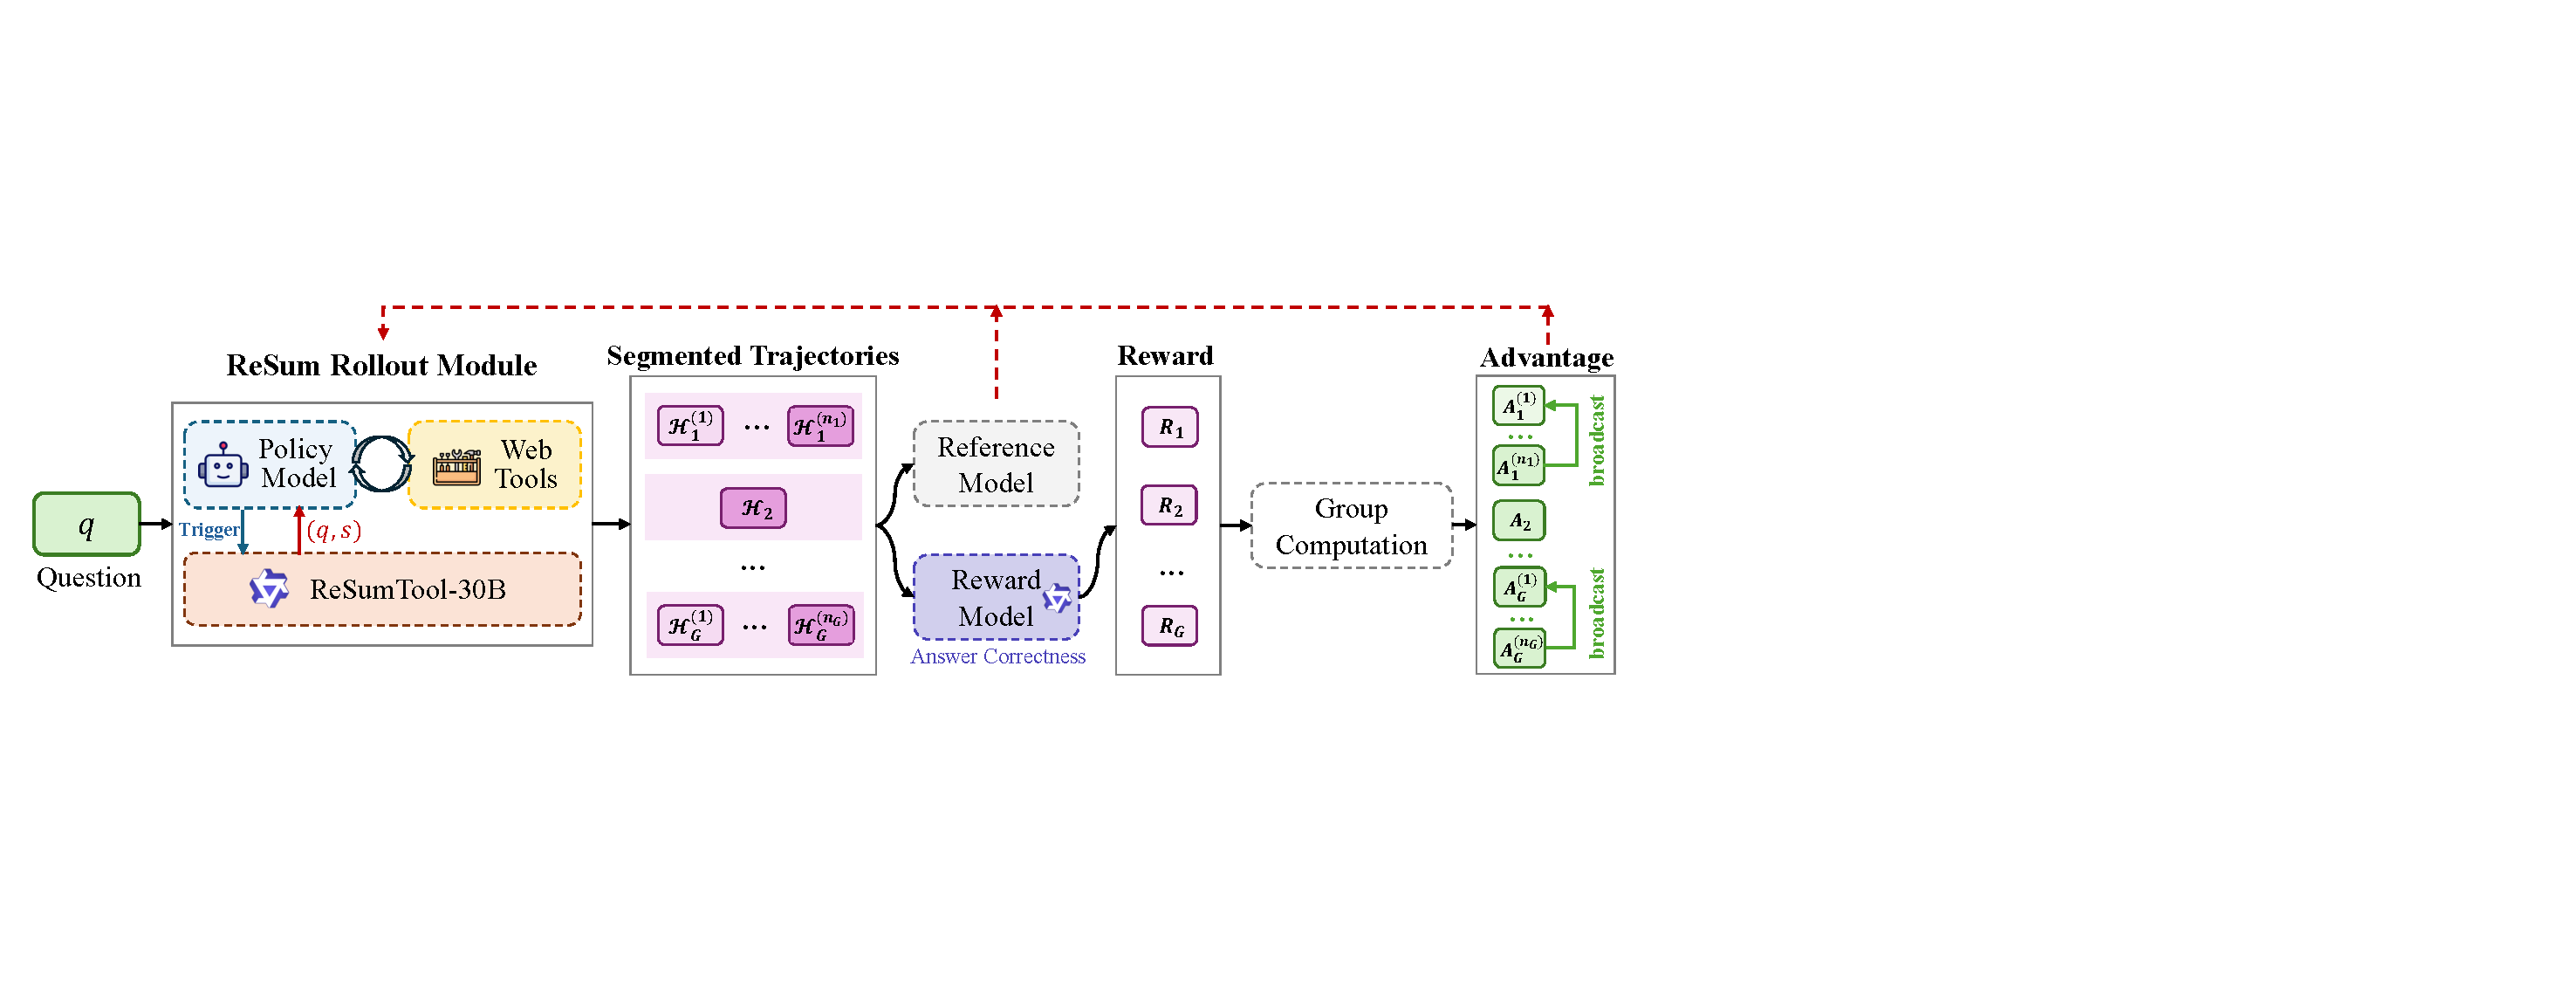
\includegraphics[width=0.9\linewidth]{images/ReSum-RL.pdf}
    \caption{\textbf{Illustration of ReSum‑GRPO.} ReSum periodically summarizes long trajectories and restarts from compressed states, resulting in segmented trajectories. A single trajectory-level reward is computed from the final answer, normalized within the group to obtain a trajectory-level advantage, and that advantage is \textbf{\textit{broadcast}} to all segments within the same rollout.}
    \label{fig:resum_grpo}
\end{figure*}

\subsection{ReSum-GRPO}
The ReSum paradigm creates a novel query type $q' = (q, s)$ that combines the original user query $q$ with a summary $s$. While agents can process such inputs, they may initially reason suboptimally from summarized contexts as this pattern was not encountered during training. Therefore, we employ RL to master such paradigm. Unlike supervised fine-tuning, which requires costly collection of expert-level ReSum trajectories and risks overwriting an agent's existing skills, RL enables agents to adapt to this paradigm through self-evolution while retaining their inherent reasoning capabilities.

\textbf{Trajectory Segmentation:} The key modification of ReSum-RL is that ReSum naturally segments long trajectories into multiple episodes when summarization occurs. Consider a complete ReSum trajectory that undergoes $K$ summarization events. This trajectory is naturally partitioned into the following $K+1$ segments:
\begin{align*}
\mathcal{H}^{(1)} &= (q^{(0)}, \tau_1, a_1, o_1, \ldots, \tau_{t_1}, a_{t_1}, o_{t_1}) \\
\mathcal{H}^{(2)} &= (q^{(1)}, \tau_{t_1+1}, a_{t_1+1}, o_{t_1+1}, \ldots, \tau_{t_2}, a_{t_2}, o_{t_2}) \\
&\vdots \\
\mathcal{H}^{(K+1)} &= (q^{(K)}, \tau_{t_K+1}, a_{t_K+1}, o_{t_K+1}, \ldots, \tau_T, a_T),
\end{align*}
where $q^{(0)} = q$ is the initial query, $q^{(k)} = (q, s^{(k)})$ is the compressed state after the $k$-th summarization, and $a_T$ denotes the final answer. Each segment $\mathcal{H}^{(i)}$ forms an individual training episode with input $q^{(i-1)}$ and output $(\tau_{t_{i-1}+1}, a_{t_{i-1}+1}, o_{t_{i-1}+1}, \ldots, \tau_{t_i}, a_{t_i})$ where all observations $o$ are masked during loss computation as they are environmental returns. For trajectories that complete without summarization, we have the degenerate case $K=0$, yielding a single segment that follows the same training format.


\textbf{Reward Computation:} To avoid manually designing per-segment rewards, we utilize a unified trajectory-level reward signal. Solely based on the final answer $a_T$ extracted from the last segment, we compute the reward $R(a^{\star}, a_T) \in \{0,1\}$ against the ground truth $a^{\star}$ using an LLM-as-Judge strategy~\citep{gu2024survey, li2024llmsasjudgescomprehensivesurveyllmbased}. This approach provides an outcome-based reward per trajectory, which can be shared across all segments if necessary. Additionally, we enforce a strict format constraint: if the agent fails to adhere to specific tokens, e.g., \lightthink{}, the entire trajectory is terminated with zero reward. Such penalty ensures strict adherence to the interaction protocol.

\textbf{GRPO Integration (Figure \ref{fig:resum_grpo}):} ReSum‑RL modifies only the rollout collection by segmenting on summaries and adjusts the reward signal to be trajectory-level answer correctness. Consequently, it is compatible with various RL algorithms~\citep{ppo,rlhf,yu2025dapo}. Specifically, we instantiate this with GRPO~\citep{shao2024deepseekmath}, resulting in ReSum‑GRPO. For an initial question $q$, we sample a group of $G$ rollouts, each producing $n_g$ segments as $\{\mathcal{H}_g^{(i)}\}_{i=1}^{n_g}$. The objective can be written as:
\begin{equation*}
\label{eq:grpo}
\begin{aligned}
\mathcal{J}_{\text{GRPO}}(\theta) = \mathbb{E} \Bigg[ & \frac{1}{\sum_{g=1}^{G}n_g} \sum_{g=1}^{G}\sum_{i=1}^{n_g} \min \bigg(  r_g^{(i)}(\theta) \hat{A}_g^{(i)}, \\
& \text{clip}\big(r_g^{(i)}(\theta), 1-\varepsilon_{\text{low}}, 1+\varepsilon_{\text{high}}\big) \hat{A}_g^{(i)} \bigg) \Bigg],
\end{aligned}
\end{equation*}
where the expectation $\mathbb{E}$ is taken over the dataset and the sampling policy as $\mathbb{E}_{(q,a^{\star}) \sim \mathcal{D},  \{ \mathcal{H}_{g}^{(i)} \}_{g=1, i=1}^{G, n_g} \sim \pi_{\theta_{\text{old}}} }$, and $r_g^{(i)}(\theta)$ is the importance sampling ratio for segment $i$ in rollout $g$. In alignment with GRPO, rather than directly broadcasting rewards, we broadcast the trajectory-level advantage. For trajectory $g$, we extract the final answer $a_{g, T}$ from its last segment and compute a trajectory‑level reward $R_g \in \{0,1\}$. This reward is then normalized within the group to obtain the advantage as $\hat{A}_g = \frac{R_g - \text{mean}(\{R_1,\dots,R_G\})}{\text{std}(\{R_1,\dots,R_G\})}$, which is broadcast to all segments within rollout $g$ as $\hat{A}_g^{(i)} = \hat{A}_g$ for $i \in \{ 1,\dots,n_g \}$. Such mechanism ensures a consistent learning signal per trajectory while leveraging GRPO’s group-wise stabilization.

In summary, the advantage broadcasting mechanism in ReSum-GRPO enables effective learning from all segments of long-horizon tasks by: (1) encouraging agents to reason successfully from compressed states, and (2) ensuring early exploration steps receive appropriate bonus when they contribute to the final success. Notably, ReSum-GRPO only modifies long trajectories by utilizing segmented rollouts, while short trajectories are processed identically to standard GRPO. This design not only maintains training efficiency but also preserves the agent’s inherent reasoning patterns.
